\documentclass[11pt]{article}
\usepackage[a4paper,margin=2.2cm]{geometry}
\usepackage{amsmath,amssymb,amsthm}
\usepackage[T1]{fontenc}
\usepackage{lmodern}
\usepackage{enumitem}
\usepackage{xcolor}
\usepackage{microtype}
\usepackage{tikz}
\usetikzlibrary{arrows.meta,positioning,fit,backgrounds}
\tikzset{
  v/.style={circle,draw,minimum size=6mm,inner sep=0pt,font=\small},
  fr/.style={fill=green!15},            % free vertex
  mv/.style={fill=blue!10},             % matched vertex
  non/.style={gray!80,thick},           % non-matching edge
  mat/.style={blue!70!black,line width=2pt},   % matching edge
  nw/.style={orange!85!black,line width=2pt},  % edge of the other matching N
  hl/.style={red!70!black,line width=1.4pt,dash pattern=on 4pt off 2pt},
  cp/.style={font=\scriptsize\itshape,inner sep=1pt,align=center},
  every picture/.style={>=Stealth},
}
\newcommand{\legend}{\par\nopagebreak\noindent{\footnotesize Legend: \textcolor{blue!70!black}{\rule[0.5ex]{1.2em}{2pt}}\,matching edge\quad \textcolor{gray}{\rule[0.5ex]{1.2em}{1pt}}\,non-matching edge\quad \colorbox{green!15}{\,free\,}\ vertex\par}}
\usepackage[colorlinks=true,linkcolor=blue!50!black]{hyperref}

\setlength{\parindent}{0pt}
\setlength{\parskip}{0.55em}

\newcounter{qe}\newcounter{qh}
\newcommand{\Qhead}[2]{%
  \vspace{0.9em}\par\noindent
  {\large\bfseries #1\ #2}\par\nopagebreak\vspace{-0.2em}}
\newcommand{\EQ}[1]{\refstepcounter{qe}\Qhead{E\theqe.}{#1}}
\newcommand{\HQ}[1]{\refstepcounter{qh}\Qhead{H\theqh.}{#1}}
\newcommand{\A}{\par\noindent\textbf{Answer.}\ }
\newcommand{\Watch}[1]{\par\noindent{\small\color{red!60!black}\textbf{Watch out:} #1}}
\newcommand{\symd}{\oplus}

\title{CS G526 -- Hopcroft--Karp\\Practice Questions for the Q\&A}
\author{}
\date{}

\begin{document}
\maketitle

\noindent Forty practice questions with answers. \textbf{Part I} (E1--E20) is the
basic set: definitions, why greedy fails, augmenting paths, the idea of a phase.
\textbf{Part II} (H1--H20) is tougher: proofs, justification of each step, and
connections to other results. Notation: $M$ is the current matching, $s$ the size
of a maximum matching, $m$ the number of edges, $n$ the number of vertices. The
length of a path is its number of edges; ``$M\symd P$'' means flipping $P$ in $M$.

The answers come from the paper (Hopcroft and Karp, SIAM J.\ Comput.\ 1973) and
standard facts. Facts that go beyond the paper were checked against the original
sources and are marked.

\tableofcontents
\newpage

\part{Basic questions}

\section{Problem, greedy, augmenting paths}

\EQ{Why is greedy wrong? Give a small counterexample.}
\A Take the path $a$--$1$, $a$--$2$, $b$--$1$. If $a$ grabs $1$, then $b$ is stuck, and
only one pair is made. The best matching is $a$--$2$, $b$--$1$. Greedy never undoes an
earlier choice.

\begin{center}
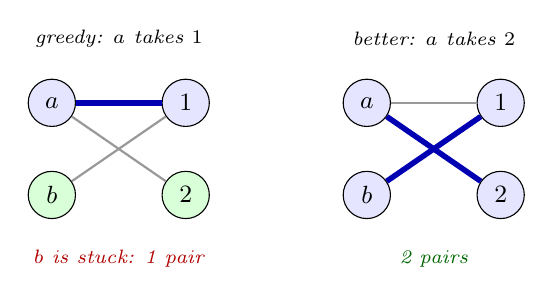
\begin{tikzpicture}[x=1.7cm,y=0.9cm]
 \begin{scope}
  \node[cp] at (0.5,0.9) {greedy: $a$ takes $1$};
  \node[v,mv] (a) at (0,0) {$a$}; \node[v,fr] (b) at (0,-1.3) {$b$};
  \node[v,mv] (1) at (1,0) {$1$}; \node[v,fr] (2) at (1,-1.3) {$2$};
  \draw[mat] (a)--(1); \draw[non] (a)--(2); \draw[non] (b)--(1);
  \node[cp,red!70!black] at (0.5,-2.2) {$b$ is stuck: 1 pair};
 \end{scope}
 \begin{scope}[xshift=4cm]
  \node[cp] at (0.5,0.9) {better: $a$ takes $2$};
  \node[v,mv] (a) at (0,0) {$a$}; \node[v,mv] (b) at (0,-1.3) {$b$};
  \node[v,mv] (1) at (1,0) {$1$}; \node[v,mv] (2) at (1,-1.3) {$2$};
  \draw[non] (a)--(1); \draw[mat] (a)--(2); \draw[mat] (b)--(1);
  \node[cp,green!40!black] at (0.5,-2.2) {2 pairs};
 \end{scope}
\end{tikzpicture}
\end{center}

\EQ{Is a maximal matching the same as a maximum matching?}
\A No. Maximal means no edge can be added. Maximum means the largest possible size.
Greedy gives a maximal matching, which is at least half the size of a maximum one.

\EQ{Why does an augmenting path always have odd length, and why must it start and end on opposite sides?}
\A Its edges alternate: non-matching, matching, \dots, non-matching. It starts and
ends at free vertices, so it has one more non-matching edge than matching edges, hence
odd length. In a bipartite graph every step switches side, so an odd number of steps
ends on the other side.


\begin{center}
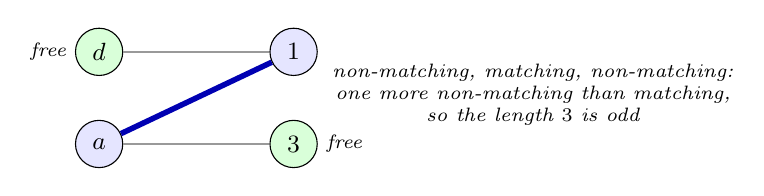
\begin{tikzpicture}[x=1.9cm,y=0.9cm]
  \node[v,fr] (d) at (0,0) {$d$}; \node[v,mv] (a) at (0,-1.3) {$a$};
  \node[v,mv] (1) at (1.3,0) {$1$}; \node[v,fr] (3) at (1.3,-1.3) {$3$};
  \draw[non] (d)--(1); \draw[mat] (1)--(a); \draw[non] (a)--(3);
  \node[cp,left=2pt of d] {free}; \node[cp,right=2pt of 3] {free};
  \node[cp] at (2.9,-0.6) {non-matching, matching, non-matching:\\one more non-matching than matching,\\so the length $3$ is odd};
\end{tikzpicture}
\end{center}
\EQ{Why does flipping an augmenting path give a valid matching, and why is it exactly one bigger?}
\A The interior vertices just swap partners, so each is still matched exactly once.
The two end vertices were free and each gains one edge. The path has one more
non-matching edge than matching edge, so the matching grows by exactly $1$.


\begin{center}
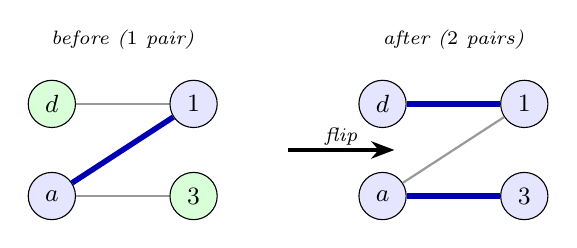
\begin{tikzpicture}[x=1.5cm,y=0.9cm]
 \begin{scope}
  \node[cp] at (0.6,0.9) {before ($1$ pair)};
  \node[v,fr] (d) at (0,0) {$d$}; \node[v,mv] (a) at (0,-1.3) {$a$};
  \node[v,mv] (1) at (1.2,0) {$1$}; \node[v,fr] (3) at (1.2,-1.3) {$3$};
  \draw[non] (d)--(1); \draw[mat] (1)--(a); \draw[non] (a)--(3);
 \end{scope}
 \draw[->,very thick] (2,-0.65)--(2.9,-0.65) node[midway,above,cp]{flip};
 \begin{scope}[xshift=4.2cm]
  \node[cp] at (0.6,0.9) {after ($2$ pairs)};
  \node[v,mv] (d) at (0,0) {$d$}; \node[v,mv] (a) at (0,-1.3) {$a$};
  \node[v,mv] (1) at (1.2,0) {$1$}; \node[v,mv] (3) at (1.2,-1.3) {$3$};
  \draw[mat] (d)--(1); \draw[non] (1)--(a); \draw[mat] (a)--(3);
 \end{scope}
\end{tikzpicture}
\end{center}
\EQ{State Berge's theorem. Why is the ``if'' direction true?}
\A A matching is maximum if and only if there is no augmenting path. Suppose $M$ is
not maximum and take a larger $N$. In $M\oplus N$ every component is a path or an
even cycle. Because $N$ is larger, some component has more $N$-edges than $M$-edges,
and that component is an augmenting path for $M$.


\begin{center}
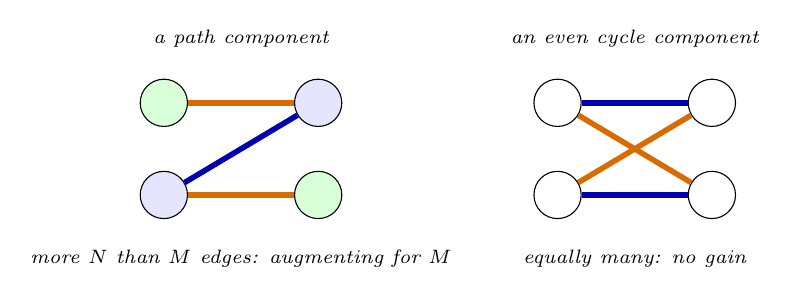
\begin{tikzpicture}[x=1.4cm,y=0.9cm]
 \node[cp] at (0.7,0.9) {a path component};
 \node[v,fr] (u1) at (0,0) {}; \node[v,mv] (u2) at (0,-1.3) {};
 \node[v,mv] (w1) at (1.4,0) {}; \node[v,fr] (w2) at (1.4,-1.3) {};
 \draw[nw] (u1)--(w1); \draw[mat] (w1)--(u2); \draw[nw] (u2)--(w2);
 \node[cp] at (0.7,-2.2) {more $N$ than $M$ edges: augmenting for $M$};
 \begin{scope}[xshift=5cm]
 \node[cp] at (0.7,0.9) {an even cycle component};
 \node[v] (x1) at (0,0) {}; \node[v] (x2) at (0,-1.3) {};
 \node[v] (y1) at (1.4,0) {}; \node[v] (y2) at (1.4,-1.3) {};
 \draw[mat] (x1)--(y1); \draw[nw] (y1)--(x2); \draw[mat] (x2)--(y2); \draw[nw] (y2)--(x1);
 \node[cp] at (0.7,-2.2) {equally many: no gain};
 \end{scope}
\end{tikzpicture}\\[2pt]
{\footnotesize \textcolor{blue!70!black}{blue} = edge of $M$, \textcolor{orange!85!black}{orange} = edge of $N$.}
\end{center}
\EQ{Does Berge's theorem need the graph to be bipartite?}
\A No, it holds in every graph. What gets harder in a general graph is \emph{finding}
an augmenting path, because of odd cycles (Edmonds' blossoms). In a bipartite graph
the search can't close an odd cycle.

\EQ{How do you find one augmenting path in $O(m)$? Why is it enough to search from the free vertices?}
\A Run a BFS or DFS from the free left vertices. Go from left to right along
non-matching edges and from right to left along matching edges. If you reach a free
right vertex, you have an augmenting path. Each vertex is visited once, so the cost is
$O(m)$. An augmenting path must begin at a free left vertex, so starting anywhere else
is pointless.

\EQ{Why is the classical algorithm $O(mn)$?}
\A There are at most $n/2$ augmentations, since each adds one pair, and each needs one
$O(m)$ search.

\EQ{How is this the same as Ford--Fulkerson?}
\A Add a source joined to every left vertex and a sink joined from every right vertex,
all with capacity $1$. A flow of value $k$ is a matching of size $k$. An augmenting
path in the residual graph is an augmenting path for the matching, and the backward
residual edge is the matched edge being undone. So the classical algorithm is
Ford--Fulkerson on this network.


\begin{center}
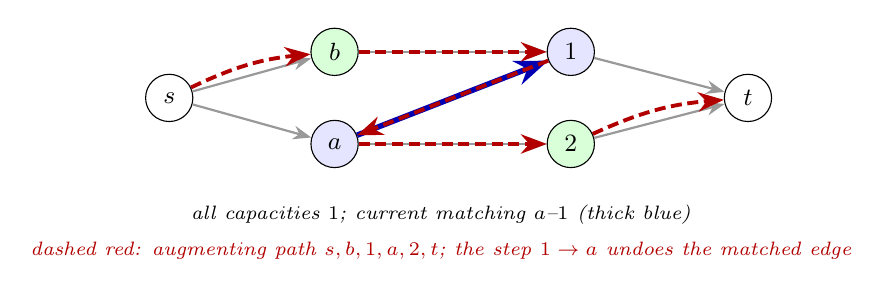
\begin{tikzpicture}[x=1.5cm,y=0.9cm]
 \node[v] (s) at (-1.4,-0.65) {$s$}; \node[v] (t) at (3.5,-0.65) {$t$};
 \node[v,fr] (b) at (0,0) {$b$}; \node[v,mv] (a) at (0,-1.3) {$a$};
 \node[v,mv] (1) at (2,0) {$1$}; \node[v,fr] (2) at (2,-1.3) {$2$};
 \draw[->,non] (s)--(b); \draw[->,non] (s)--(a);
 \draw[->,non] (b)--(1); \draw[->,non] (a)--(2); \draw[->,mat] (a)--(1);
 \draw[->,non] (1)--(t); \draw[->,non] (2)--(t);
 \draw[->,hl] (s) to[bend left=10] (b); \draw[->,hl] (b)--(1);
 \draw[->,hl] (1) to (a);              \draw[->,hl] (a)--(2); \draw[->,hl] (2) to[bend left=10] (t);
 \node[cp] at (0.9,-2.3) {all capacities $1$; current matching $a$--$1$ (thick blue)};
 \node[cp,red!70!black] at (0.9,-2.8) {dashed red: augmenting path $s,b,1,a,2,t$; the step $1\to a$ undoes the matched edge};
\end{tikzpicture}
\end{center}
\EQ{Can the same idea be used directly on a general (non-bipartite) graph?}
\A Not directly. Odd cycles confuse the search, since a vertex can be reached at
both even and odd depth. Edmonds' blossom algorithm shrinks them. Micali and Vazirani
(FOCS 1980) obtained the Hopcroft--Karp bound $O(m\sqrt{n})$ for general graphs. The
paper itself only hopes for such an extension.

\section{The Hopcroft--Karp idea}

\EQ{Why shortest augmenting paths? Why not just any set of disjoint paths?}
\A Shortest paths are what make the lengths grow from phase to phase (Theorem 2). With
arbitrary paths nothing forces the shortest length to grow, so there is no clean bound
on the number of phases.

\EQ{Why does the shortest augmenting path length strictly increase after a phase?}
\A After a phase the chosen set is maximal, so no augmenting path of the old shortest
length is left that avoids the chosen paths. Theorem 2 says a new path $P'$ satisfies
$|P'|\ge|P|+2|P\cap P'|$. If $P'$ is disjoint from all of them it would have been
addable, contradicting maximality; if it overlaps, it is longer. Lengths are odd, so
the new shortest length is at least $2$ more.

\EQ{Why is the length always odd, and where does the ``$+2$'' come from?}
\A Augmenting paths in a bipartite graph have odd length. A strictly larger odd number
is at least $2$ larger.

\EQ{Walk me through the $\sqrt{n}$ argument in plain words.}
\A After $\sqrt{n}$ phases the shortest augmenting path has length at least $\sqrt{n}$.
By Berge's theorem the gap to the maximum equals the number of vertex-disjoint
augmenting paths still available, and each of those uses at least $\sqrt{n}$ vertices.
There are only $n$ vertices, so there are at most $n/\sqrt{n}=\sqrt{n}$ such paths.
Each remaining phase adds at least one pair, so at most $\sqrt{n}$ more phases are
needed. Total: about $2\sqrt{n}$.

\EQ{Why must the paths in one phase be vertex-disjoint?}
\A If two paths shared a vertex, flipping both would give that vertex two partners.
Disjointness is what lets us flip them all at once. It is also automatic for equal-length
shortest paths found one after another (H4).

\EQ{What does the BFS do, and what does the DFS add?}
\A The BFS gives every vertex its distance from the free left vertices and keeps only
the edges that go from layer $i$ to layer $i+1$. Every path in this layered graph is a
shortest path. The DFS then picks a maximal set of vertex-disjoint paths from it. It
deletes vertices it has used or found useless, so each edge is scanned only once.


\begin{center}
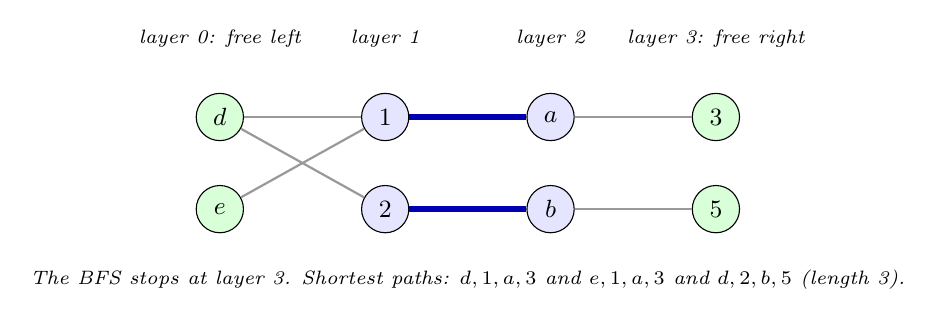
\begin{tikzpicture}[x=2.1cm,y=0.9cm]
 \foreach \i/\t in {0/{layer 0: free left},1/{layer 1},2/{layer 2},3/{layer 3: free right}} \node[cp] at (\i,1.1) {\t};
 \node[v,fr] (d) at (0,0) {$d$}; \node[v,fr] (e) at (0,-1.3) {$e$};
 \node[v,mv] (1) at (1,0) {$1$}; \node[v,mv] (2) at (1,-1.3) {$2$};
 \node[v,mv] (a) at (2,0) {$a$}; \node[v,mv] (b) at (2,-1.3) {$b$};
 \node[v,fr] (3) at (3,0) {$3$}; \node[v,fr] (5) at (3,-1.3) {$5$};
 \draw[non] (d)--(1); \draw[non] (d)--(2); \draw[non] (e)--(1);
 \draw[mat] (1)--(a); \draw[mat] (2)--(b);
 \draw[non] (a)--(3); \draw[non] (b)--(5);
 \node[cp] at (1.5,-2.3) {The BFS stops at layer 3. Shortest paths: $d,1,a,3$ and $e,1,a,3$ and $d,2,b,5$ (length 3).};
\end{tikzpicture}
\end{center}
{\small Example: matching $\{a1,b2,c4\}$ from our running example, after the first phase. Vertices $c$ and $4$ are never reached.}
\EQ{Why is a phase $O(m)$ and not more?}
\A The BFS visits each edge once. In the DFS every vertex is either used on a path or
deleted after a dead end, so each edge is examined a constant number of times.

\EQ{Why is the total $O(m\sqrt{n})$? What was the bound in the paper?}
\A There are $O(\sqrt{n})$ phases and each costs $O(m)$. The paper states $O(n^{5/2})$,
which is the same bound for dense graphs, where $m$ can be about $n^2$.

\EQ{Is a phase's set of paths maximal or maximum? Does a phase find all augmenting paths of that length?}
\A Maximal. After the phase no further vertex-disjoint augmenting path of that
length can be added, but a different scan order would give a different set of paths.
What is guaranteed is only that the next shortest length is strictly larger.

\EQ{Is $O(m\sqrt{n})$ the best known? What came after?}
\A For bipartite matching in sparse graphs it is still the classical bound, but there
is later work. Even and Tarjan (1975) showed Dinic's algorithm runs in
$O(m\sqrt{n})$ on ``unit'' networks (every vertex except the source and sink has
in-degree $1$ or out-degree $1$), which covers bipartite matching. Micali and Vazirani
(1980) got $O(m\sqrt{n})$ for general graphs. Chen, Kyng, Liu, Peng, Probst Gutenberg
and Sachdeva (FOCS 2022) gave max-flow in $m^{1+o(1)}$ time, which also solves
bipartite matching. None of this is in the Hopcroft--Karp paper; I checked it against
the original sources.

\part{Tougher questions}

%--------------------------------------------------------------------
\section{Structure and the basic lemmas}

\HQ{Why is every component of $M\symd N$ a path or an even cycle?}
\A Take two matchings $M$ and $N$. Every vertex has at most one $M$-edge and at
most one $N$-edge, so in $M\symd N$ it has degree at most $2$. A graph of maximum
degree $2$ is a disjoint union of paths and cycles. Along a component the edges
must alternate between $M$ and $N$, because two edges of the same matching can't
meet at a vertex. A cycle that alternates has even length. In a bipartite graph
this is automatic anyway, since every cycle is even.

\HQ{Prove: if $|M|=r<s=|N|$, then $M\symd N$ contains at least $s-r$ vertex-disjoint
augmenting paths relative to $M$.}
\A Look at each component of $M\symd N$. An even cycle has equally many $M$ and $N$
edges. A path has $|N|-|M|\in\{-1,0,1\}$ among its edges. Summing over components,
the total is $|N|-|M|=s-r$. So at least $s-r$ components have one more $N$-edge
than $M$-edge. Such a component is a path that starts and ends with $N$-edges, and
its end vertices are not covered by $M$ (otherwise the path would continue along
an $M$-edge). So it is an augmenting path relative to $M$. Different components
share no vertices.

\Watch{say ``relative to $M$''. The same paths are alternating for $N$ in the other direction.}

\HQ{After a phase, why can't the next shortest augmenting path be as short as the old one? Prove Theorem 2 from scratch.}
\A Theorem 2 says: if $P$ is a shortest augmenting path for $M$ and $P'$ is
augmenting for $M\symd P$, then $|P'|\ge |P|+2\,|P\cap P'|$.

Let $N=M\symd P\symd P'$. Then $|N|=|M|+2$, since each flip adds one edge. By the
previous question, $M\symd N=P\symd P'$ contains two vertex-disjoint augmenting
paths $P_1,P_2$ relative to $M$. Since $P$ is shortest for $M$, each has length at
least $|P|$. Their edges are inside $P\symd P'$, so
\[
2|P|\le|P_1|+|P_2|\le |P\symd P'|=|P|+|P'|-2|P\cap P'|.
\]
Rearranging gives $|P'|\ge|P|+2|P\cap P'|$. The paper states the weaker
$|P'|\ge|P|+|P\cap P'|$. The proof gives the factor $2$.

\HQ{Use that to show augmenting along shortest paths one at a time gives non-decreasing lengths, and that equal lengths force vertex-disjointness.}
\A Non-decreasing: $|P'|\ge|P|+2|P\cap P'|\ge|P|$.

Equal lengths: suppose $|P'|=|P|$, so $|P\cap P'|=0$ edges. Suppose they still
shared a vertex $v$. After flipping $P$, every vertex of $P$ is matched by an
edge of $P$. If $v$ is an end of $P'$, it must be free, a contradiction. If $v$ is
interior to $P'$, $P'$ uses the matching edge at $v$, which is an edge of $P$.
That makes $|P\cap P'|\ge1$, a contradiction. So equal-length paths are
vertex-disjoint. This is exactly why a phase can take all the shortest paths at
once.

\HQ{Prove: if $M$ has size $r$ and a maximum matching has size $s$, the shortest augmenting path for $M$ has length at most $2\lfloor r/(s-r)\rfloor+1$.}
\A There are at least $s-r$ vertex-disjoint augmenting paths (H2). Each uses some
edges of $M$, and the $M$-edges of different paths are different. So the total
number of $M$-edges on them is at most $r$. By pigeonhole, one of them has at most
$\lfloor r/(s-r)\rfloor$ matching edges. An augmenting path with $k$ matching edges
has length $2k+1$. Hence the bound.

\section{The $\sqrt{n}$ phase bound}

\HQ{Give the full argument that the number of phases is $O(\sqrt{s})$.}
\A Split the phases into two groups.

\emph{First $\lceil\sqrt{s}\rceil$ phases.} The shortest length is odd and strictly
increases, starting at $1$. So after $k$ phases it is at least $2k+1$.

\emph{After that.} Let $M$ be the matching at that point, of size $r$. Its
shortest augmenting path has length at least $2\lceil\sqrt{s}\rceil+1\ge2\sqrt{s}+1$.
The bound of the previous question says that length is at most
$2\lfloor r/(s-r)\rfloor+1$. So $r/(s-r)\ge\sqrt{s}$, which gives
$s-r\le r/\sqrt{s}\le s/\sqrt{s}=\sqrt{s}$. At most $\sqrt{s}$ augmentations are
left, and every phase does at least one. Total: at most about $2\sqrt{s}$ phases.

\HQ{Strictly increasing by one would give only $\sqrt{s}$ phases at best. Why do we need the increase to be at least $2$?}
\A Two reasons. Paths in a bipartite graph have odd length, so the next
possible length after $2k+1$ is $2k+3$. That is what lets us say the length after
$k$ phases is at least $2k+1$. If we only knew it grows by $1$ per phase, we would
get $k+1$, and the second group would leave up to about $2\sqrt{s}$ augmentations
instead of $\sqrt{s}$. This changes only the constant, not the $O(\sqrt{s})$, but
the claim ``grows by one'' (as in the video you watched) is simply false in a
bipartite graph: it grows by at least $2$.

\HQ{Does the phase bound depend on $n$ or on $s$? What if $|X|\ne|Y|$?}
\A It depends on $s$, the size of the maximum matching: about $2\sqrt{s}+2$
phases. Since $s\le\min(|X|,|Y|)\le n/2$, this is $O(\sqrt{n})$. An unbalanced
graph only helps. The proof does not need $|X|=|Y|$.

\HQ{Is the $\sqrt{n}$ bound on phases tight? Do you know a graph family that forces it?}
\A The paper proves an upper bound and I have not verified a matching lower bound
from the paper. I would not claim one. What I can say is that the analysis is
tight for the argument as written, and that in practice the number of phases is
usually very small. If asked, say so honestly instead of guessing.

\Watch{this is a ``don't bluff'' question. A clear ``I don't know, the paper doesn't say'' is better than a guess.}

\HQ{Could we start from a greedy matching? Does the bound change?}
\A Yes, we may start from any matching, including the empty one. The proof uses
only $s$ and the fact that lengths are odd and strictly increase. So the bound
$\approx2\sqrt{s}+2$ holds from any starting point. A greedy start usually saves
several phases in practice, but it doesn't change the worst-case bound.

\section{The phase itself}

\HQ{Why does the BFS stop at the first layer that contains a free vertex on the right?}
\A That layer gives the length of the shortest augmenting paths. Anything found
further out would be longer, and we promised to use only shortest paths. If we
continued, Theorem 2 would no longer apply to the paths we pick, and the length
could stay the same from one phase to the next.

\HQ{Why can the DFS ignore edges inside a layer or going backwards?}
\A A shortest augmenting path visits vertices in increasing distance from the free
vertices on the left. Each step moves from layer $i$ to layer $i+1$. A step that
stays in a layer or goes back would make the path longer than the BFS distance,
so it can't be on a shortest path. So the layered graph contains every shortest
augmenting path and nothing else.

\HQ{Justify the deletion rules in the DFS. Why is deleting a dead-end vertex safe, and why is deleting a used vertex safe?}
\A \emph{Dead end.} If every outgoing edge of $v$ has been tried and failed, no
path through $v$ reaches a free vertex. Since the graph only loses vertices, that
stays true. So $v$ is useless for the rest of the phase.

\emph{Used vertex.} Once a path has been printed, its vertices are matched
differently now, and later paths in this phase must be vertex-disjoint from it.
So they can't use those vertices, and removing them is exactly what we want.

Because every vertex is deleted at most once and each edge is scanned only when
its tail is examined, the DFS costs $O(m)$.

\HQ{At the end of a phase, what exactly do we know? Is it a maximal or a maximum set of paths?}
\A Maximal. No further vertex-disjoint augmenting path of the current shortest
length can be added. It is not the maximum possible set, and different scan orders
give different sets. What does not depend on the order is the next phase's shortest
length, which is strictly bigger.

\HQ{Could we pick vertex-disjoint paths that aren't all of the shortest length, say any maximal disjoint set of augmenting paths? Would the proof survive?}
\A No. Theorem 2 needs $P$ to be a shortest path. If we allow longer paths, the
shortest length need not grow after the phase, so we lose the first group of the
$\sqrt{s}$ argument. I would not claim a lower bound on the running time for that
variant. I can only say the proof breaks.

\section{Connections and extensions}

\HQ{What does the final failed search tell you? Link it to K\"onig's theorem.}
\A When no augmenting path remains, the search from the free left vertices reaches
a set $S$. Let $L$ be the left vertices reached and $R$ the right vertices
reached. Then $(X\setminus L)\cup R$ is a vertex cover, and it has size equal to
$|M|$ (each cover vertex is matched, and no matching edge has both ends in it).
So the maximum matching equals the minimum vertex cover, which is K\"onig's
theorem. The algorithm gives a certificate of optimality for free.


\begin{center}
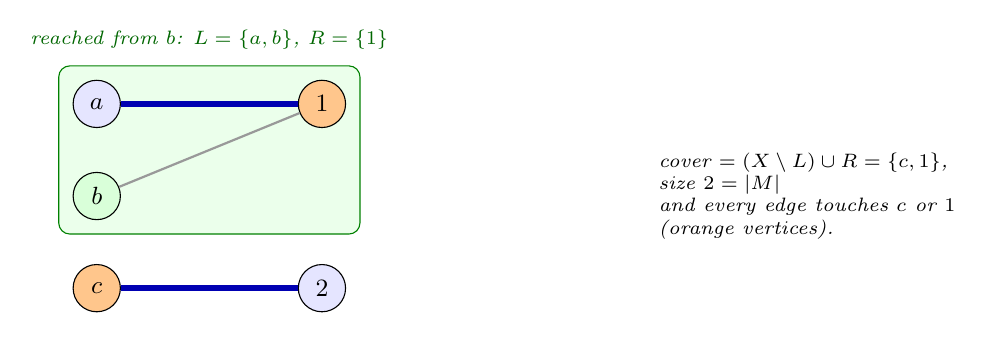
\begin{tikzpicture}[x=2.2cm,y=0.9cm]
 \node[v,mv] (a) at (0,0) {$a$}; \node[v,fr] (b) at (0,-1.3) {$b$}; \node[v,mv,fill=orange!45] (c) at (0,-2.6) {$c$};
 \node[v,mv,fill=orange!45] (1) at (1.3,0) {$1$}; \node[v,mv] (2) at (1.3,-2.6) {$2$};
 \draw[mat] (a)--(1); \draw[non] (b)--(1); \draw[mat] (c)--(2);
 \begin{scope}[on background layer]
  \node[draw=green!50!black,rounded corners,fill=green!8,fit=(a)(b)(1),inner sep=5pt] {};
 \end{scope}
 \node[cp,green!40!black] at (0.65,0.9) {reached from $b$: $L=\{a,b\}$, $R=\{1\}$};
 \node[cp,align=left] at (4.1,-1.3) {cover $=(X\setminus L)\cup R=\{c,1\}$,\\ size $2=|M|$ \\ and every edge touches $c$ or $1$\\ (orange vertices).};
\end{tikzpicture}
\end{center}
\HQ{When there is no perfect matching, how does the algorithm give you a Hall violator?}
\A Run it until it stops. If some left vertex $u$ is still free, search from it. The
set $L$ of left vertices reached has neighbourhood exactly the set $R$ of right
vertices reached. Every vertex of $R$ is matched, to a vertex of $L\setminus\{u\}$,
so $|R|=|L|-1<|L|$. That is a violation of Hall's condition.


In the example of the previous figure, the free vertex is $b$, the reached set is
$L=\{a,b\}$, and $N(L)=\{1\}$. So $|N(L)|=1<2=|L|$: no matching can cover both $a$ and $b$.
\HQ{State the relation to maximum flow precisely. Where does the $\sqrt{n}$ come from in flow terms?}
\A Build the network with source $s$, sink $t$, and unit capacities. Integer flows
correspond to matchings. Augmenting paths in the residual graph correspond to
augmenting paths for the matching. A phase of Hopcroft--Karp is the same as one
blocking-flow phase of Dinic's algorithm on this network. The network is
``unit'': every vertex other than $s,t$ has in-degree $1$ or out-degree $1$.
Even and Tarjan (SIAM J.\ Comput.\ 4(4), 1975) showed Dinic runs in $O(m\sqrt{n})$
on such networks. This is not in the Hopcroft--Karp paper; I checked it against
the Even--Tarjan abstract. Careful: for networks that only have unit \emph{capacities}
their bound is the weaker $O(\min(n^{2/3},m^{1/2})\,m)$. The $\sqrt{n}$ needs the
``every inner vertex has in- or out-degree 1'' structure.

\HQ{Can Hopcroft--Karp be used for \emph{weighted} bipartite matching?}
\A Not directly. ``Shortest'' here means fewest edges, not least weight. For
maximum-weight or min-cost matching you need the Hungarian method or min-cost
flow, because an augmenting path must be chosen to keep the weights optimal.
Cardinality matching is the special case where all weights are equal.

\HQ{Where does the bipartite assumption get used? What goes wrong in a general graph?}
\A It is used in two places. First, to say augmenting paths have odd length, which
gives the $+2$ in the length growth. Second, in the search: from the left side you
only reach the right side by non-matching edges, so the layers are clean. In a
general graph an odd cycle can make the same vertex reachable at both even and odd
depth, and the BFS labelling breaks. Edmonds' blossom algorithm handles that by
contracting odd cycles; Micali and Vazirani (FOCS 1980) showed that the $O(m\sqrt{n})$ bound
also holds there, though a complete proof appeared later (Vazirani, arXiv:2012.03582).
The paper ends by hoping for such an extension.

\end{document}
